\documentclass[parskip=full]{scrartcl}
\usepackage[top=2.54cm, bottom=2.54cm, left=2.54cm, right=2.54cm]{geometry}
\usepackage[utf8]{inputenc} % use utf8 file encoding for TeX sources
\usepackage[T1]{fontenc}    % avoid garbled Unicode text in pdf
\usepackage[ngerman]{babel}  % german hyphenation, quotes, etc
\usepackage{hyperref}       % hyperlinks in document
\usepackage{glossaries}     % glossary 
\usepackage{enumerate}      % advanced enumeration
\usepackage[shortlabels]{enumitem}
\usepackage[dvipsnames]{xcolor}
\usepackage{graphicx}
\usepackage{caption}        % add captions
\usepackage{adjustbox}      % add adjustmentbox
\usepackage{csquotes}

% Set footer and header bar
\usepackage[headsepline, footsepline]{scrlayer-scrpage}
\addtokomafont{headsepline}{\color{BlueViolet}}
\addtokomafont{footsepline}{\color{BlueViolet}}
\KOMAoptions{headsepline=1.25pt:\textwidth}
\KOMAoptions{footsepline=1.25pt:\textwidth}
\clearpairofpagestyles
\rofoot{\thepage}
\ihead{Write your own Android App: SpiceSquad}

% set the hyperlink style in the document
\hypersetup{
    pdftitle={PSE: Pflichtenheft},
    pdfborderstyle={/S/U/W 1},
    colorlinks,
    linkcolor={black!50!black},
    citecolor={blue!50!black},
    urlcolor={blue!80!black}
}

% sets right quotation for "
\MakeOuterQuote{"}

%change figure numbering
\renewcommand{\thefigure}{\thesection.\arabic{figure}}

%add command to hide subsections from toc
\newcommand{\changelocaltocdepth}[1]{%
  \addtocontents{toc}{\protect\setcounter{tocdepth}{#1}}%
  \setcounter{tocdepth}{#1}%
}

\newcommand{\resetSubSectionNumbering}{
    \renewcommand{\thesubsection}{\arabic{section}.\arabic{subsection}}
    \changelocaltocdepth{3} 
}

% glossary
\makeglossaries
\renewcommand{\glossarysection}[2][]{}

\begin{document}
\newglossaryentry{label}{
    name=Label,
    plural=Labels,
    description={Rezepte können mit bezeichnenden Stichwörtern, sogenannten Labels, versehen werden. Dies ermöglicht das Filtern von Rezepten nach bestimmten Eigenschaften (z.B. vegetarisch, glutenfrei, halal)}
}

\begin{titlepage}
    \begin{center}
        \begin{Huge}
            {\textbf{Write your own Android App: SpiceSquad}}
        \end{Huge}
        \vspace{12px}

        Praxis der Softwareentwicklung (PSE)\\
        Sommersemester 2023\\
        \vspace{150px}

        \begin{Huge}
            {\textbf{Pflichtenheft}}
        \end{Huge}
        \vspace{12px}

        \textbf{Auftraggeber}\\
        Karlsruher Institut für Technologie\\
        KASTEL — Institut für Informationssicherheit und Verlässlichkeit\\
        \vspace{330px}

        \textbf{Auftragnehmer}\\
        Karlsruher Intellektuelle\\
        Henri Becker, Konrad Knappe, Lukas Schwarz, Raphael Zipperer\\
    \end{center}
\end{titlepage}

\tableofcontents
\newpage

\section*{Gender-Hinweis}
Zur besseren Lesbarkeit wird in diesem Pflichtenheft das generische Maskulinum verwendet.
Die in diesem Heft verwendeten Personenbezeichnungen beziehen sich – sofern nicht anders kenntlich gemacht – auf alle Geschlechter.
\newpage

\section{Zielbestimmung}
\subsection{Musskriterien}
Musskriterien: unabdingbare Leistungen der Software.

\begin{enumerate}[start=1,label={$\langle$\bfseries RM\arabic*$\rangle$}, leftmargin = 5em, itemsep=4pt, parsep=4pt]
    \item Der Nutzer muss sich mit einer E-Mail-Adresse, einem Nutzernamen und einem Passwort registrieren können.\label{rm:Registering}
    \item Der registrierte Nutzer muss sich mit seiner E-Mail-Adresse und seinem Passwort anmelden, um auf die Funktionen der App zugreifen zu können. \label{rm:Login}
    \item Der angemeldete Nutzer muss sich abmelden können. \label{rm:Logout}
    \item Der Nutzer muss eine Gruppe erstellen können. \label{rm:GroupCreation}
    \item In jeder Gruppe muss mindestens ein Gruppenadmin sein, der nach Erstellung nur der Ersteller ist.\label{rm:GroupAdmin}
    \item Der Gruppenadmin kann die Gruppe auflösen. \label{rm:GroupDeletion}
    \item Der Nutzer einer Gruppe mithilfe eines Gruppenkürzels beitreten können und diese danach auch wieder verlassen können.\label{rm:GroupJoining}
    \item Der Nutzer muss Rezepte erstellen und hochladen können.\label{rm:RecipeCreation}
    \item Der Nutzer muss zu jedem Rezept den Rezepttitel, die Zubereitungsdauer, die Zutaten mit Mengenangaben, den Schwierigkeitsgrad, die Portionsanzahl und eine Zubereitungsanweisungen angeben können.\label{rm:RecipeContents}
    \item Nutzer können Rezepte von allen Erstellern in der gleichen Gruppe anschauen können.\label{rm:RecipeViewing}
    \item Der Rezeptersteller muss seine Rezepte separat ändern und löschen können.\label{rm:RecipeManagement}
    \item Jedes Gruppenmitglied muss das Gruppenkürzel einsehen können.\label{rm:GroupId}
\end{enumerate}

\subsection{Sollkriterien}
Sollkriterien: Leistungen, die enthalten sein sollten, bei Bedarf jedoch auch weggelassen werden können.

\begin{enumerate}[start=1,label={$\langle$\bfseries RS\arabic*$\rangle$}, leftmargin = 5em, itemsep=4pt, parsep=4pt]
    \item Der Nutzer soll bei Rezepten Portionen skalieren können.\label{rs:PortionScaling}
    \item Der Nutzer soll Rezepte favorisieren können.\label{rs:RecipeFavourites}
    \item Der Nutzer soll die \Gls{sichtbarkeit} der von ihm erstellten Rezepte ändern können.\label{rs:RecipeVisibility}
    \item Ein Administrator soll Gruppenmitglieder zum Administrator ernennen und den Administratorenstatus wieder entziehen können.\label{rs:AdminCreation}
    \item Ein Administrator soll Nutzer aus Gruppen \Gls{kicken} und \Gls{bannen} können.\label{rs:Kicking}
    \item Ein Administrator soll Rezepte von anderen Nutzern in der Gruppe ausblenden können.\label{rs:RecipeHiding}
    \item Das Hinzufügedatum und der Benutzername des Erstellers eines Rezeptes soll einsehbar sein.\label{rs:AuthorAndDate}
    \item Der Nutzer soll sein Passwort wieder zurücksetzen können, indem er einen Link an seine E-Mail-Adresse geschickt bekommt.\label{rs:ResetPassword}
    \item Der Nutzer soll sein Konto nach erstellen wieder löschen können.\label{rs:AccountDeletion}
    \item Der Nutzer soll das Gruppenkürzel auch über einen QR-Code teilen können.\label{rs:QRCode}
    \item Der Nutzer soll seinen Nutzernamen ändern können.\label{rs:ChangeUsername}
    \item Der Nutzer kann nach Rezepten anhand ihres Titels suchen.\label{rs:Searching}

\end{enumerate}

\subsection{Kannkriterien}
Kannkriterien: Leistungen, die umgesetzt werden können, falls noch Zeit ist.

\begin{enumerate}[start=1,label={$\langle$\bfseries RC\arabic*$\rangle$}, leftmargin = 5em, itemsep=4pt, parsep=4pt]
    \item Der Nutzer kann Rezepte in Form von PDFs exportieren.\label{rc:PDFExport}
    \item Der Nutzer kann genau ein Bild zu jedem Rezept hochladen.\label{rc:Images}
    \item Der Nutzer kann Zutaten aus einer Liste auswählen.\label{rc:IngredientList}
    \item Der Nutzer kann sein Profilbild ändern.\label{rc:ProfileImage}
    \item Der Nutzer kann Rezepte nach Favoriten und Schwierigkeitsgrad filtern.\label{rc:Filtering}
    \item Der Nutzer kann Rezepte jeweils auf- und absteigend Alphabetisch nach dem Namen des Rezepts, nach dem Schwierigkeitsgrad und dem Hinzufügedatum sortieren.\label{rc:Sorting}
    \item Nur ein Administrator kann den Gruppennamen ändern.\label{rc:GroupRenaming}
    \item Der Administrator kann die Gruppe verlassen und das frühste Mitglied der Gruppe wird automatisch neuer Administrator.\label{rc:AdminLeaves}
    \item Der Nutzer kann ein Rezept dem Administrator melden.\label{rc:RecipeMelden}

\end{enumerate}

\subsection{Abgrenzungskriterien}
Abgrenzungskriterien: Leistungen die explizit nicht umgesetzt werden.

\begin{enumerate}[start=1,label={$\langle$\bfseries RW\arabic*$\rangle$}, leftmargin = 5em, itemsep=4pt, parsep=4pt]
    \item Es gibt keine Möglichkeit Rezepte durch Kommentare zu
    \item Der Nutzer kann keine Rezepte bewerten.
    \item Es gibt keine integrierte Chatfunktion.
    \item Das Hinzufügen von Videos zu den Rezepten ist nicht
    \item Über die App kann man keine anderen Nutzer direkt suchen.
    \item Es existiert kein Gruppenprofilbild.
    \item Der Nutzer kann nicht zwischen Dark Mode und Light Mode wechseln.
\end{enumerate}

\section{Produkteinsatz}
Dieses Kapitel dient dazu, den Einsatzbereich, die Zielgruppen und die Betriebsbedingungen der zu entwickelnden Software aufzuführen.

\subsection{Anwendungsbereiche}
In diesem Abschnitt wird erläutert, in welchen Bereichen die Software eingesetzt werden soll. \newline
Die App bietet eine Reihe von Funktionen, die Nutzern eine Vielzahl an Anwendungsmöglichkeiten rund um das Thema kochen bieten.
Zum einen können Nutzer Rezepte hochladen und diese bei Bedarf im Nachhinein bearbeiten.
Dies ermöglicht das Teilen von Rezepten mit anderen Nutzern. Eigene Rezepte können außerdem auf privat gestellt werden, sodass nur der erstellende Nutzer selbst diese sehen kann.
Die App kann also auch als eine Art digitales Kochbuch benutzt werden, um eigene Rezepte zu organisieren und bei Bedarf auch von anderen Geräten aufrufen zu können.
Nutzer können außerdem Kochgruppen, sogenannten \Gls{squad}, beitreten, um Rezepte mit Nutzern mit ähnlichen Interessen zu teilen und die öffentlichen Rezepte anderer Nutzer in diesen Gruppen zu betrachten. Nutzer können die Rezepte ihrer Gruppen nach bestimmten Kriterien filtern, sortieren und suchen. So können Nutzer gezielt ihre Kochkenntnisse erweitern.
Rezepte können zudem skaliert werden, um die richtige Menge für eine bestimmte Anzahl an Personen effizient zu ermitteln.

\subsection{Zielgruppen}
Im Folgenden wird aufgezählt, für welche Anwender die Software im Wesentlichen gedacht ist. \newline
Die Koch App richtet sich an alle, die gerne kochen und ihre Kocherfahrung verbessern möchten.
Die App ist insbesondere für Gruppen geeignet, in denen gekocht wird (Bsp. Wohngemeinschaften), da Rezepte effizient geteilt und skaliert werden können.

\subsection{Betriebsbedingungen}
In diesem Unterkapitel wird auf die unterschiedlichen Bedürfnisse und Anforderungen an die Software eingegangen. \newline
Um die volle Funktionsfähigkeit der App garantieren zu können, ist eine Internetverbindung erforderlich. Außerdem können QR-Codes für Gruppen nur mit einer funktionierenden Handykamera gescannt werden, auf die die App zugreifen kann.

\section{Produktübersicht}

In diesem Kapitel werden die Produktfunktionen beschrieben und in einem Use-Case-Diagramm "Aufbau der App" visualisiert.
Das Use-Case-Diagramm zeigt mittels Verbindungslininen, wie die einzelnen Use-Cases zueinander stehen.
Die Hauptansicht wird genauer im Aktivitätsdiagramm "Hauptansicht" abgebildet.
Die Gruppen-Detail-Ansicht als Administrator wird in einem weiteren Aktivitätsdiagramm "Gruppen-Detail-Ansicht als Administrator" dargestellt und erläutert.

Dadurch können die einzelnen Schritte, die durchlaufen werden, besser beschrieben werden.\par


\paragraph{Aufbau der App (\autoref{fig:UseCaseDiagram}):}

In dem Use-Case-Diagramm „Aufbau der App“ sieht man die allgemeine Struktur der App. 

Bei der erstmaligen Nutzung muss der Nutzer sich registrieren.

Dazu muss er seinen Benutzernamen, seine E-Mail-Adresse und ein Passwort eingeben.
Das Passwort muss durch eine erneute Eingabe bestätigt werden.
Nach Bestätigung der Eingabe kann der Nutzer eine Gruppe erstellen, einer Gruppe beitreten oder diesen Punkt überspringen und erstmal keiner Gruppe beitreten.
Durch das erstellen einer Gruppe wird man automatisch zum Administrator der Gruppe.
Der Nutzer kann einer Grupppe durch Eingabe eines Gruppenkürzels oder durch scannen eines QR-Codes beitreten.
Der Nutzer kann eine Gruppe durch Eingabe eines Gruppennamens erstellten.

Falls der Nutzer schon ein Nutzerkonto besitzt kann er sich einloggen.
Dazu muss er seine E-Mail-Adresse und sein Passwort eingeben.
Hat der Nutzer sein Passwort vergessen besteht die Möglichkeit das Passwort zurückzusetzen.
Ein eingeloggter Nutzer muss sich nicht erneut einloggen.\newline
Nach dem Einloggen gelangt der Nutzer auf die Hauptansicht.
Hier hat er die Möglichkeit, Rezepte zu filtern, favorisieren, suchen oder zu sortieren.
Durch klicken auf ein Rezept gelangt der Nutzer auf der Rezeptansicht.
Die Rezeptansicht wird unter dem Aktivitätsdiagramm "Hauptansicht" (Abbildung 3.2) noch genauer beschrieben.
Durch klicken auf den Rezept-erstellen-Button gelangt der Nutzer auf der Rezept-Erstellungs-Ansicht.
Hier kann der Nutzer ein neues Rezept erstellen.
Es können Zutaten, Zubereitungsanweisung, Schwierigkeitgrad und Kochzeit ƒür das neue Rezept angegeben werden.

Im Anschluss kann das Rezept veröffentlicht werden.\par
Durch klicken auf den Verwaltungs-Ansicht-Button
gelangt der Nutzer auf die Verwaltungs-Ansicht.
In dieser Ansicht kann der Nutzer sich ausloggen, sein Nutzerkonto löschen, seinen Nutzernamen ändern,
erstellte Rezepte bearbeiten, eine Gruppe verlassen und Gruppen-Kürzel oder Gruppen-QR-Codes teilen.\par
Durch das Drücken des Gruppen-hinzufügen-Button kann der Nutzer eine neue Gruppe erstellen oder beitreten.

Von der Verwaltungs-Ansicht kommt der Nutzer durch klicken auf eine Gruppe auf die Gruppen-Detail-Ansicht.
Eingeloggte Nutzer können hier Gruppenmitglieder und Rezepte von Gruppenmitgliedern einsehen, die Gruppe verlassen oder den QR-Code zum beitreten der Gruppe einsehen.
Durch das klicken auf die Rezepte gelangt der Nutzer auf die Rezeptansicht des dazugehörigen Rezepts.
Gruppenadministratoren können in dieser Ansicht Gruppenmitglieder entfernen, bannen, zum Administrator ernennen, als Administrator entfernen, Rezepte von Gruppenmitgliedern für die Gruppe ausblenden oder die Gruppe auflösen.\par



\paragraph{Hauptansicht (\autoref{fig:ActivityDiagramMainView}):}

Im Aktivitätsdiagramm „Hauptansicht“
werden die verschiedenen Möglichkeiten unter dem Menüpunkt Hauptansicht aufgeführt.


Der Nutzer hat die Möglichkeit Rezepte durch eine Suchfeld zu suchen.
Der Nutzer hat die Möglichkeit die Liste durch vorgegebene Sortierungen zu sortieren oder nach Filterkriterien zu filtern.
Vorgegeben Sortierungen sind auf- oder absteigend Alpahbetisch nach Namen des Rezepts, nach dem Schwierigkeitsgrad und nach dem Hinzufügedatum.
Die Liste lässt sich nach Favoriten oder Schwierigkeitsgrad filtern.
Es besteht zudem die Möglichkeit Rezepte schon in dieser Ansicht zu favorisieren.\newline
Beim Auswählen eines Rezepts öffnet sich die dazugehörige Rezeptansicht.
In dieser Ansicht kann der Nutzer das Rezept ansehen, favorisieren und die Portionsgrößen ändern.
Es besteht zudem die Möglichkeit Rezepte zu melden.
Ist der Nutzer der Ersteller des Rezept hat er zudem die Möglichkeit das Rezept zu bearbeiten.
Wird ein Rezept gemeldet, so werden die Administratoren mit einer E-Mail auf die Meldung benachrichtigt.\newline
Es be
Durch klicken auf zurück gelangt der Nutzer wieder auf der Hauptansicht.\par


\paragraph{Gruppen-Detail-Ansicht als Administrator (\autoref{fig:ActivityDiagramAdmin}):}

Im Aktivitätsdiagramm "Gruppen-Detail-Ansicht als Administrator" wir gezeigt, welche Möglichkeiten der Nutzer als Administrator einer Gruppe in der "Gruppen-Detail-Ansicht" hat.

Der Administrator muss in der Verwaltungsansicht die Gruppe wählen in der er Gruppenadministrator ist.
Der Administrator landet so in der Gruppen-Detail-Ansicht.
Durch klicken auf ein Rezept kann der Gruppenadministrator, eingeblendete Rezepte ausblenden und ausgeblendete Rezepte einblenden.\newline
Beim Auswählen von Gruppenmitgliedern gibt es die Möglichkeit das Gruppenmitglied zu entfernen oder zu bannen.
Der Administrator muss die jeweilige Aktion nachträglich nochmal bestätigen.
Ein entfernter Nutzer kann der Gruppe wieder beitreten wohingegen ein gebannter Nutzer der Gruppe unwiderruflich nicht mehr beitreten kann.
Ein Administrator kann ein Gruppenmitglied zu einem Administrator ernennen
Ein Administrator kann einen anderen Administrator als Administrator entfernen.

Der Administrator einer Gruppe kann durch eine nachfolgende Bestätigung die Gruppe verlassen.
Ist anschließend kein weiteres Mitglied mehr in der Gruppe wird die Gruppe aufgelöst. Ein Nutzer kann der Gruppe anschließend nicht mehr beitreten.
Falls es keinen Administrator mehr in der Gruppe gibt, wird der Nutzer, der nach dem Administrator die Gruppe beigetreten ist und noch in der Gruppe ist, zum neuen Administrator.
Ein Administrator kann eine Gruppe durch eine nachfolgende Bestätigung auflösen. Ein Nutzer kann der Gruppe anschließend nicht mehr beitreten.\newline
Der Administrator kann das Gruppenkürzel durch "Gruppenkürzel kopieren" in die Zwischenablage kopieren. Der Administrator kann den QR-Code der Gruppe durch "QR-Code anzeigen" anschauen.

\newpage

\begin{figure}[!htp]
    \centering
    \begin{adjustbox}{right=160mm}
        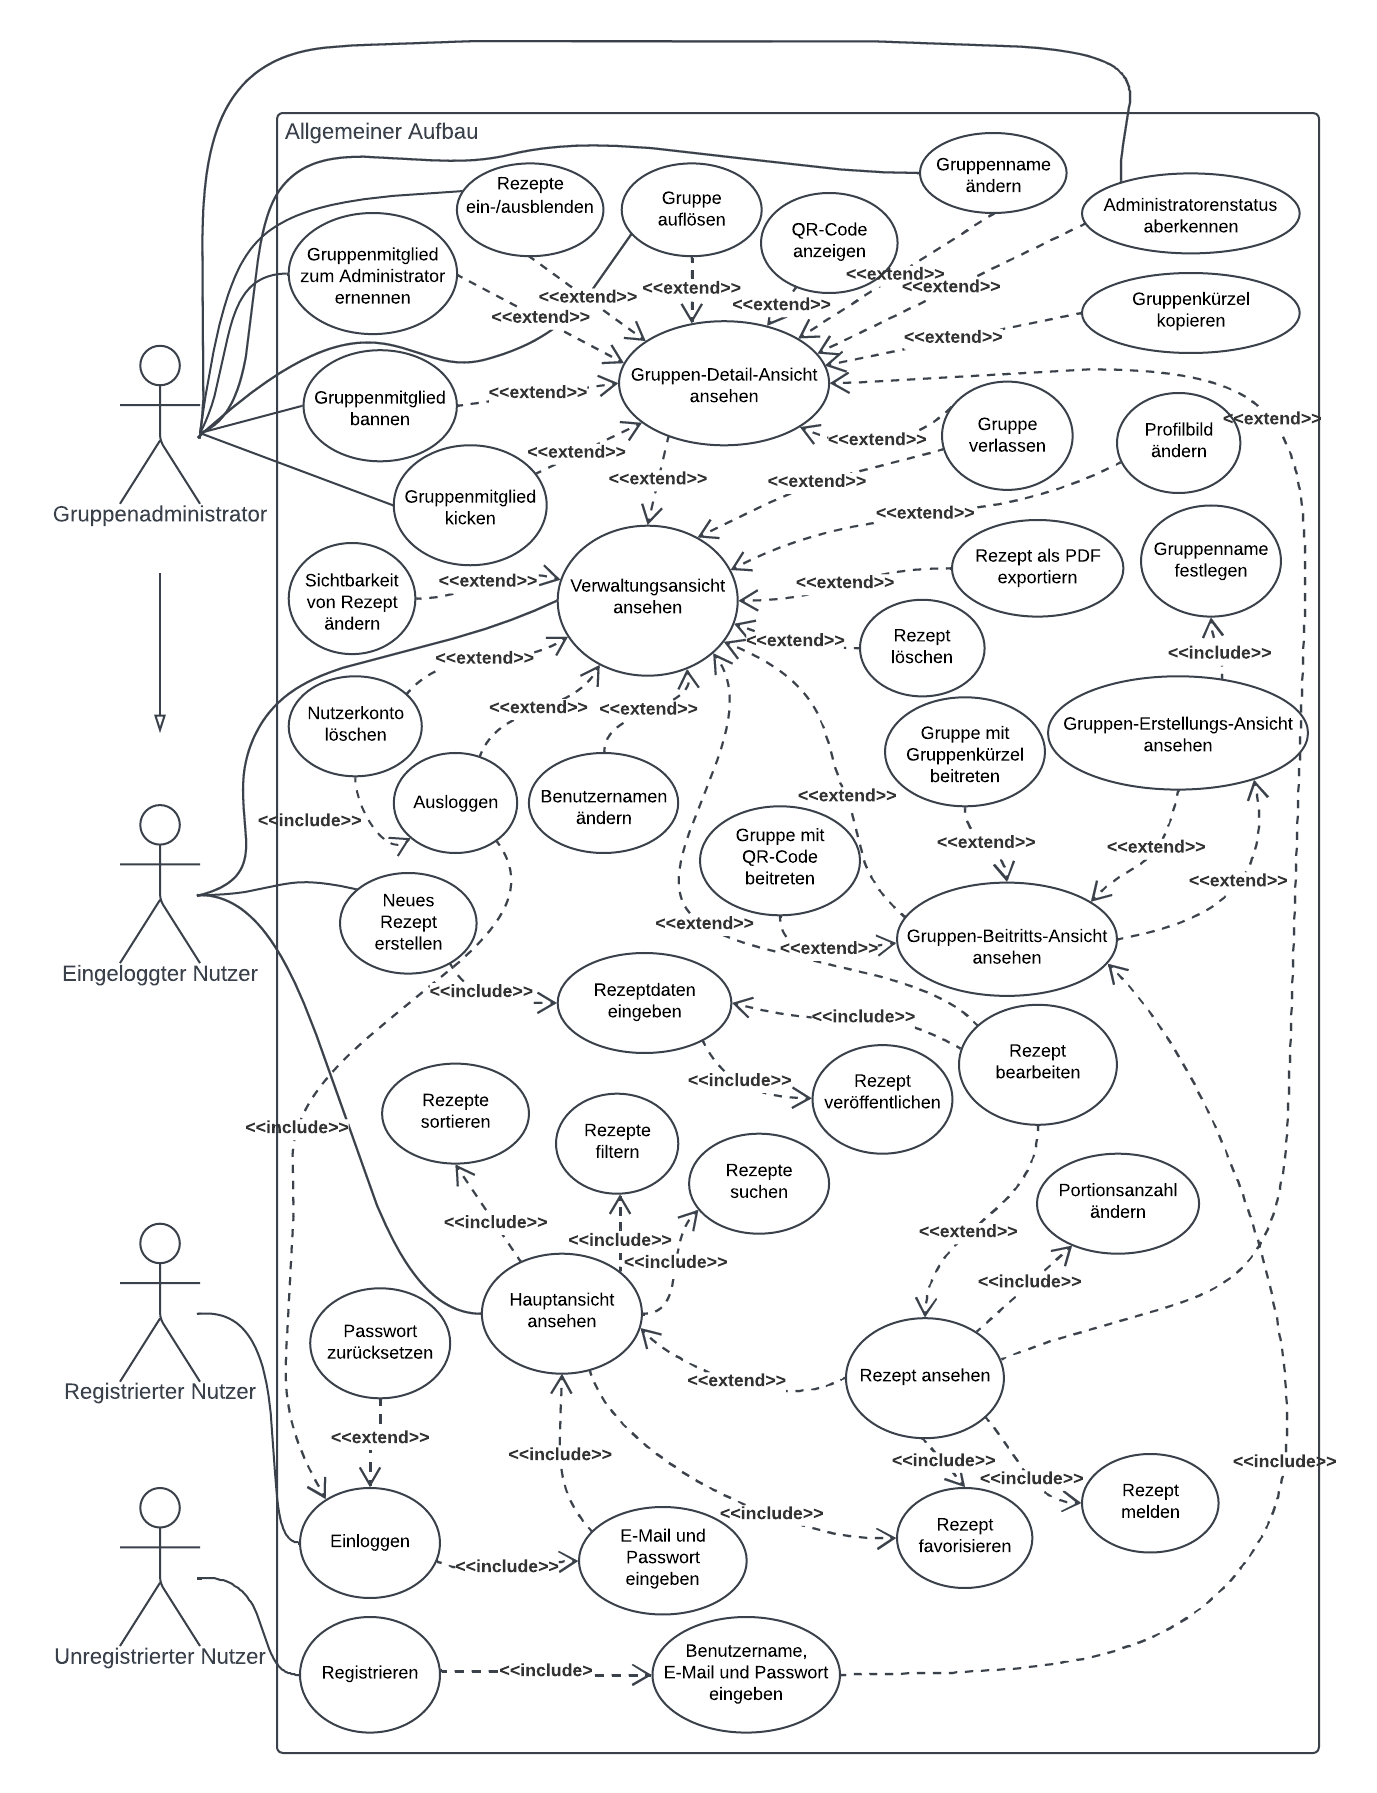
\includegraphics[height=220mm]{images/produktübersicht/UseCaseDiagram.png}
    \end{adjustbox}
    \caption{Use-Case-Diagramm: Aufbau der App}
    \label{fig:UseCaseDiagram}
\end{figure}
\newpage

\begin{figure}[!htp]
    \centering
    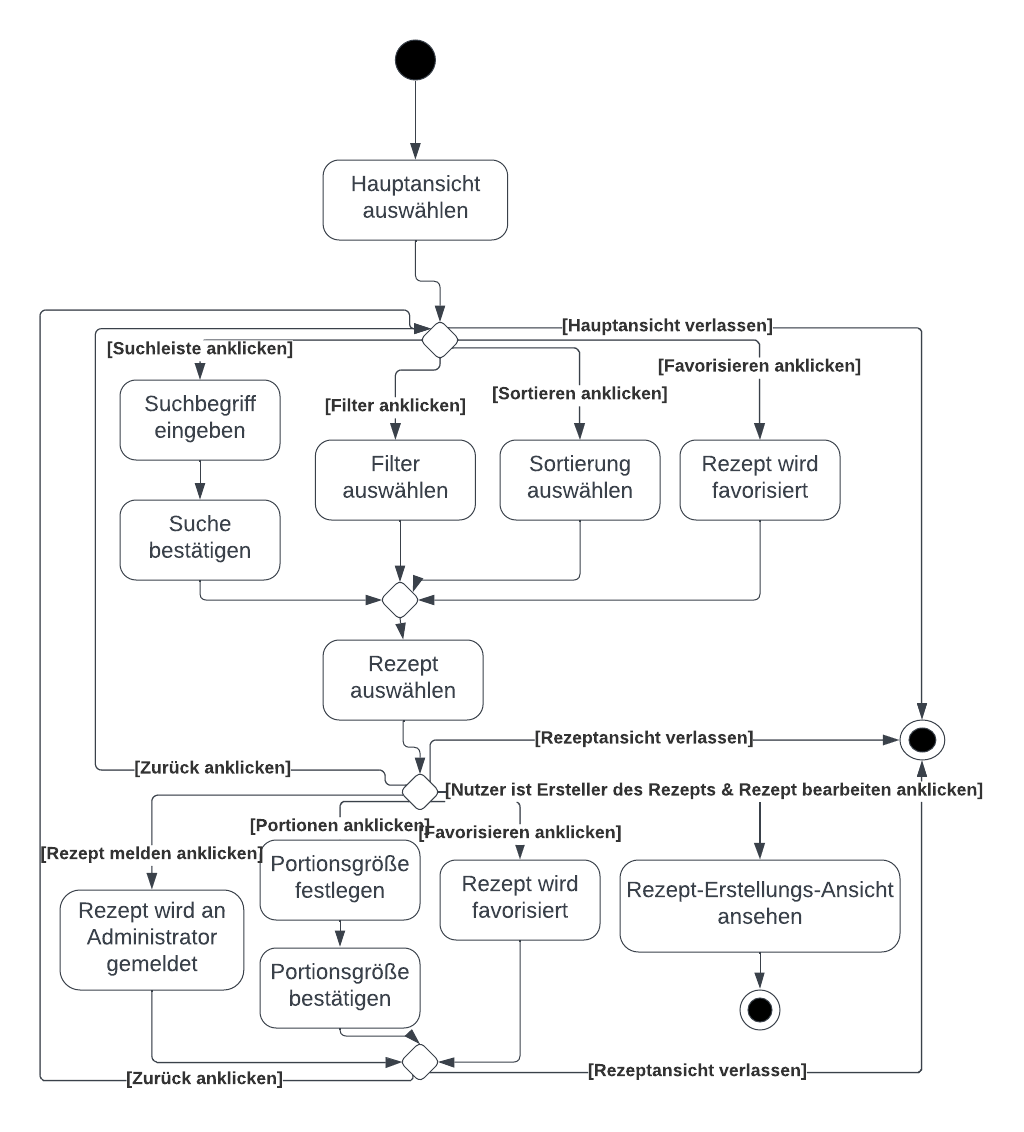
\includegraphics{images/produktübersicht/ActivityDiagramMainView.png}
    \caption{Aktivitätsdiagramm: Haupt-Ansicht}
    \label{fig:ActivityDiagramMainView}
\end{figure}
\newpage

\begin{figure}[!htp]
    \centering
    \begin{adjustbox}{right=150mm}
        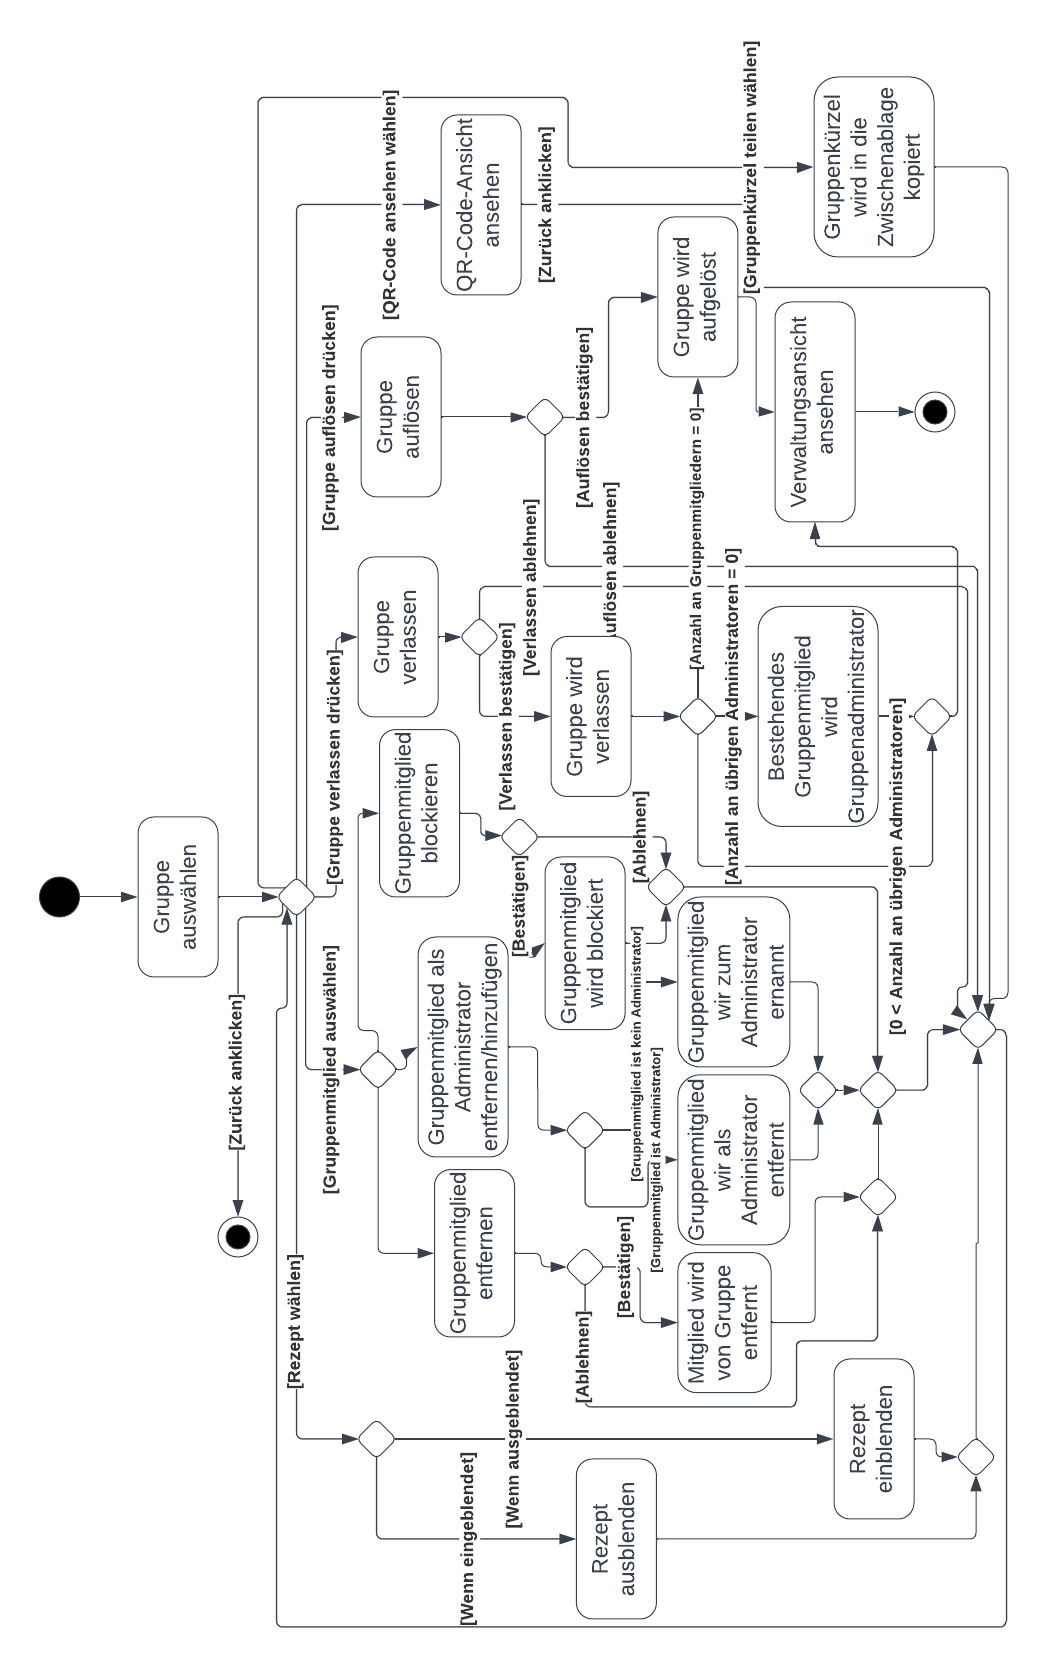
\includegraphics[height=230mm]{images/produktübersicht/ActivityDiagramAdmin.png}
    \end{adjustbox}

    \caption{Aktivitätsdiagramm: Gruppen-Detail-Ansicht als Administrator}
    \label{fig:ActivityDiagramAdmin}
\end{figure}
\newpage

\section{ Benutzeroberfläche }
\setcounter{secnumdepth}{6}
\renewcommand{\theparagraph}{$\langle$UI\arabic{paragraph}$\rangle$}

In diesem Kapitel wird die Benutzerberfläche erläutert. Es wird auf die Darstellung der einzelnen Funktionen sowie die Navigation zwischen diesen eingegangen. Alle hier gezeigten Abbildungen dienen lediglich der Veranschaulichung und sind nicht als fertige Entwürfe zu verstehen.

\paragraph*{Benutzeroberfläche:}
Bei der App handelt es sich um eine Anwendungssoftware für Android-Endgeräte. Die Benutzer-oberfläche stellt daher einen wichtigen Teil des Produktes dar. Diese muss intuitiv und einfach zu bedienen sein, um eine möglichst hohe Benutzerfreundlichkeit zu gewährleisten. Außerdem sollte sie möglichst ansprechend gestaltet sein, um den Nutzer zu motivieren, die App zu verwenden. Beides wurde im UI-Entwurf berücksichtigt. Durch eine geringe Anzahl an gut strukturierten Ansichten und eine klare Farbgebung wird eine einfache Bedienbarkeit gewährleistet. Wichtige Buttons werden durch eine auffällige Farbe hervorgehoben, um die Navigation zu erleichtern. Nun sollen die einzelnen Ansichten erläutert werden. 

\paragraph{Registrieren-Ansicht:}
\label{ui:RegisterView}
Beim Öffnen der App gelangt der Nutzer auf die Registrieren-Ansicht (\autoref{fig:RegisterView}). Hier kann er sich mit seiner E-Mail-Adresse, einem Nutzernamen und einem Passwort registrieren. Nach erfolgreicher Registrierung gelangt der Nutzer auf die Gruppen-Beitritts-Ansicht \ref{ui:GroupJoiningView}. Alternativ kann der Nutzer auch auf die Login-Ansicht \ref{ui:LoginView} wechseln.

\paragraph{Anmelde-Ansicht:}
\label{ui:LoginView}
In der Anmeldeseite (\autoref{fig:LoginView}) kann ein bereits registrierter Nutzer sich mit seiner E-Mail-Adresse und seinem Passwort anmelden. Nach erfolgreicher Anmeldung gelangt der Nutzer auf die Haupt-Ansicht \ref{ui:MainView}. Alternativ kann der Nutzer auch auf die Registrieren-Ansicht \ref{ui:RegisterView} wechseln.
Hat ein Nutzer sein Passwort vergessen, so kann er zur Passwort-Zurücksetzen-Ansicht \ref{ui:PasswordResetView} wechseln.

\paragraph{Passwort-Zurücksetzen-Ansicht:}
\label{ui:PasswordResetView}
Hier (\autoref{fig:PasswordResetView}) kann der Nutzer sein Password zurücksetzen lassen, indem er seine E-Mail-Adresse eingibt. Durch Betätigen des Weiter-Buttons bekommt er eine E-Mail zugeschickt, in der sich ein Link befindet, mit dem er ein neues Passwort vergeben kann. Außerdem wird er in der App auf die Anmelde-Ansicht \ref{ui:LoginView} weitergeleitet.

\paragraph{Gruppen-Beitritts-Ansicht:}
\label{ui:GroupJoiningView}
In dieser Ansicht (\autoref{fig:GroupJoiningView}) kann der Nutzer einer bereits bestehenden Gruppe beitreten. Dazu kann er entweder ein Gruppen-Kürzel eingeben oder mit Hilfe der Handykamera einen QR-Code scannen. In dieser Ansicht gibt es einige Unterschiede, je nachdem ob der Nutzer nach der Registrierungs-Ansicht \ref{ui:RegisterView} oder von der Verwaltungs-Ansicht \ref{ui:SettingsView} auf diese Seite gelangt. Im ersten Fall gibt es noch einen Überspringen-Knopf, mit dem der Nutzer keiner Gruppe beitritt, sondern direkt auf die Haupt-Ansicht \ref{ui:MainView} gelangt. Dorthin wird er auch weitergeleitet, wenn er einer Gruppe beigetreten ist. Im zweiten Fall gibt es einen Zurück-Knopf, mit dem der Nutzer auf die Verwaltungs-Ansicht \ref{ui:SettingsView} zurückgelangt. Das ist auch der Fall, nachdem er einer Gruppe beigetreten ist.
Alternativ kann der Nutzer auch eine Gruppe erstellen, indem er zur Gruppen-Erstellungs-Ansicht \ref{ui:GroupCreationView} wechselt.

\paragraph{Gruppen-Erstellungs-Ansicht:}
\label{ui:GroupCreationView}
In dieser Ansicht (\autoref{fig:GroupCreationView}) kann der Nutzer eine neue Gruppe erstellen. Dazu muss er einen Gruppennamen eingeben. Durch Betätigen des Weiter-Buttons wird die Gruppe erstellt und der Nutzer wieder je nach vorheriger Ansicht auf die Haupt-Ansicht \ref{ui:MainView} oder die Verwaltungs-Ansicht \ref{ui:SettingsView} weitergeleitet. Auch hier gibt es einen Zurück- oder Überspringen-Button, der so wie in \ref{ui:GroupJoiningView} funktioniert.

\paragraph{Haupt-Ansicht:}
\label{ui:MainView}
In der Haupt-Ansicht (\autoref{fig:MainView}) kann der Nutzer alle Rezepte aus den Gruppen, in denen er Mitglied ist, sehen. Diese kann er nach verschiedenen Faktoren filtern und sortieren. Durch eine Suchleiste kann er außerdem schnell ein gewünschtes Rezept finden. Jedes Rezept wird hier mit Titel, dem Bild, Kochdauer und Schwierigkeitsgrad abgebildet. Durch einen Klick auf das Herzsymbol wird ein Rezept zu den Favoriten hinzugefügt bzw. wieder entfernt. Klickt ein Nutzer auf ein Rezept, so gelangt er zur Rezept-Ansicht \ref{ui:RecipeView}.

Unten am Bildschirm befindet sich eine Navigationsleiste, die es dem Nutzer ermöglicht, zwischen verschiedenen Ansichten zu wechseln. Durch einen Klick auf das Haus-Symbol gelangt der Nutzer auf die Haupt-Ansicht \ref{ui:MainView}. Durch einen Klick auf das Notizblock-Symbol gelangt der Nutzer auf die Rezept-Erstellungs-Ansicht \ref{ui:RecipeCreationView}. Durch einen Klick auf das Personen-Symbol gelangt der Nutzer auf die Verwaltungs-Ansicht \ref{ui:SettingsView}.

\paragraph{Rezept-Ansicht:}
\label{ui:RecipeView}

In der Rezept-Ansicht (\autoref{fig:RecipeView}) wird ein bestimmtes Rezept angezeigt. Es werden der Name, das Bild, die Zutaten, die Zubereitungsanweisungen, die Kochdauer, der Schwierigkeitsgrad, der Ersteller und das Erstellungsdatum angezeigt. Der Nutzer kann durch anpassen der Portionenzahl automatisch die Zutatenmengen errechnen lassen. Durch einen Klick auf das Herzsymbol wird ein Rezept zu den Favoriten hinzugefügt bzw. wieder entfernt. Ist der Nutzer der Ersteller des Rezepts, so wird oben ein Stiftsymbol angezeigt. Durch einen Klick auf dieses Symbol gelangt der Nutzer auf die Rezept-Erstellungs-Ansicht \ref{ui:RecipeCreationView}, die bereits mit dem Rezept befüllt ist. Dort kann er das Rezept bearbeiten. Unten am Bildschirm ist wieder die Navigationsleiste, wie in \ref{ui:MainView}, zu finden. Außerdem kann der Nutzer wieder zurück zur vorherigen Ansicht gelangen, indem er auf das Zurück-Symbol oben links klickt.


\paragraph{Rezept-Erstellungs-Ansicht}
\label{ui:RecipeCreationView}
In dieser Ansicht (\autoref{fig:RecipeCreationView}) kann ein Nutzer ein neues Rezept erstellen oder ein Bestehendes bearbeiten. Dazu gibt es verschiedene Eingabefelder, die der Nutzer ausfüllen kann. Diese umfassen den Rezeptnamen, Dauer und Schwierigkeitsgrad sowie die Zubereitungsanweisungen. Zusätzlich muss der Nutzer festlegen, für wie viele Portionen das Rezept ausgelegt ist. Außerdem kann er ein Bild mit Hilfe des betriebssystemeigenen Dateimanagers hochladen, indem er auf das Bild-Symbol klickt.
Die Zutaten können mit einem Klick auf das Plus-Symbol hinzugefügt werden. Dazu öffnet sich die Zutaten-auswahl-Ansicht \ref{ui:IngredientPickerView}, in der der Nutzer die Zutat auswählen kann. Die bereits hinzugefügten Zutaten werden in einer Liste angezeigt und können durch einen Klick auf das Kreuz-Symbol entfernt werden. Ganz unten befindet sich ein Knopf zum Speichern des Rezepts. Mit diesem wird der Nutzer auf die Haupt-Ansicht \ref{ui:MainView} weitergeleitet. Bearbeitet der Nutzer eines seiner Rezepte und erstellt kein neues, so gibt es einen Zurück-Button, mit dem er auf die vorherige Ansicht gelangt. Auch hier gibt es wieder die Navigationsleiste aus \ref{ui:MainView}.

\paragraph{Zutaten-Auswahl-Ansicht:}
\label{ui:IngredientPickerView}
In dieser Ansicht (\autoref{fig:IngredientPickerView}) kann der Nutzer Zutaten erstellen. Dazu schreibt er den Namen der Zutat in das Eingabefeld und wählt Einheit und Menge aus. Während der Nutzer die Zutat eingibt sollen automatisch Zutaten gesucht werden, die zum bisher geschriebenen Text passen und als Vorschlag unter dem Eingabefeld angezeigt werden. Durch Klick auf so einen Vorschlag wird der Zutatenname auf diesen Vorschlag gesetzt. Der Nutzer hat außerdem die Möglichkeit ein Icon für die Zutat aus einem Dropdownmenü zu wählen. Durch den Hinzufügen-Button gelangt der Nutzer zurück zur Rezept-Erstellungs-Ansicht \ref{ui:RecipeCreationView}, wo die Zutat hinzugefügt wurde.
In dieser Ansicht (\autoref{fig:IngredientPickerView}) kann der Nutzer Zutaten erstellen. Dazu schreibt er den Namen der Zutat in das Eingabefeld und wählt Einheit und Menge aus. Während der Nutzer die Zutat eingibt sollen automatisch Zutaten gesucht werden, die zum bisher geschriebenen Text passen und als Vorschlag unter dem Eingabefeld angezeigt werden. Durch Klick auf so einen Vorschlag wird der Zutatenname auf diesen Vorschlag gesetzt. Der Nutzer hat außerdem die Möglichkeit ein Icon für die Zutat aus einem Dropdownmenü zu wählen. Durch den Hinzufügen-Button gelangt der Nutzer zurück zur Rezept-Erstellungs-Ansicht \ref{ui:RecipeCreationView}, wo die Zutat hinzugefügt wurde.


\paragraph{Verwaltungs-Ansicht:}
\label{ui:SettingsView}

Die Verwaltungs-Ansicht dient der Verwaltung des Nutzers, seiner Gruppen und seiner Rezepte. Der Nutzer kann seinen Anzeigenamen und sein Profilbild ändern. Zudem kann er Gruppen verlassen, in dem er auf das Kreuz-Symbol neben der entsprechenden Gruppe drückt. Durch das Plus-Symbol gelangt der Nutzer zur Gruppen-Beitritts-Ansicht \ref{ui:GroupJoiningView} in der er einer Gruppe beitreten kann oder eine neue Gruppe erstellen kann. Drückt ein Nutzer auf eine der Gruppen, so kommt er zur Gruppen-Detail-Ansicht \ref{ui:GroupDetailView}. Außerdem sieht der Nutzer seine erstellten Rezepte, die er hier mit dem entsprechenden Button entfernen, als PDF exportieren oder auf privat stellen kann. Durch Klick auf das Rezept wird man zur entsprechenden Rezept-Ansicht \ref{ui:RecipeView}.
Zudem kann der Nutzer sich ausloggen mit dem Symbol oben rechts. Daraufhin wird er zur Anmelde-Ansicht \ref{ui:LoginView} weitergeleitet. Er kann außerdem sein Konto auflösen, woraufhin er ebenfalls zur Anmelde-Ansicht \ref{ui:LoginView} geleitet wird. Auch hier gibt es wieder die Navigationsleiste aus \ref{ui:MainView}.

\paragraph{Gruppen-Detail-Ansicht:}
\label{ui:GroupDetailView}

In der Gruppen-Detail-Ansicht (\autoref{fig:GroupDetailView}) kann der Nutzer die Mitglieder und Rezepte einer Gruppe ansehen. Durch den QR-Code-Button gelangt er zur QR-Code-Ansicht \ref{ui:QRCodeView}. Durch Klick auf das Verlassen-Symbol kann die Gruppe verlassen werden. Mit dem Plus-Symbol neben der Mitglieder-Sektion wird das Gruppenkürzel in die Zwischenablage kopiert und kann geteilt werden. Durch Klick auf ein Rezept wird der Nutzer zur entsprechenden Rezept-Ansicht \ref{ui:RecipeView} weitergeleitet. Als Administrator hat man zudem die Möglichkeit die Gruppe aufzulösen, woraufhin der Nutzer wieder auf die Verwaltungs-Ansicht \ref{ui:SettingsView} gelangt. Zudem kann er Nutzer aus der Gruppe entfernen, bannen oder zu Administratoren ernennen bzw. diesen Titel wieder aberkennen. Außerdem kann er Rezepte für alle Gruppenmitglieder außer dem Ersteller verstecken bzw. wieder einblenden. Weiterhin kann er den Gruppennamen ändern, indem er auf das Stift-Symbol drückt. Auch hier gibt es wieder die Navigationsleiste aus \ref{ui:MainView}.


\paragraph{QR-Code-Ansicht:}
\label{ui:QRCodeView}
In der QR-Code-Ansicht (\autoref{fig:QRCodeView}) wird der QR-Code einer Gruppe angezeigt. Durch den Zurück-Button kommt der Nutzer zurück zur Gruppen-Detail-Ansicht (\ref{ui:GroupDetailView}). Auch hier gibt es wieder die Navigationsleiste aus \ref{ui:MainView}.
\newpage
\newpage
\subsection*{Abbildungen}
\begin{figure}[htp]
    \begin{minipage}
        [t]{0.49\textwidth}
        \centering
        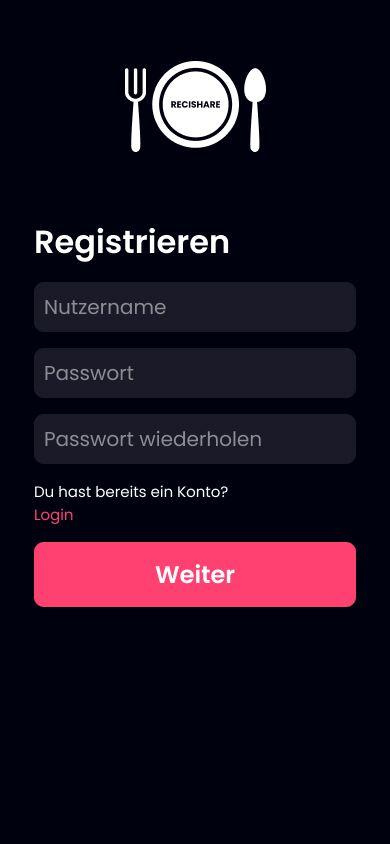
\includegraphics[height=80mm]{images/benutzeroberfläche/RegisterView.jpg}
        \caption{Registrieren-Ansicht \ref{ui:RegisterView}}
        \label{fig:RegisterView}
    \end{minipage}
    \begin{minipage}
        [t]{0.49\textwidth}
        \centering
        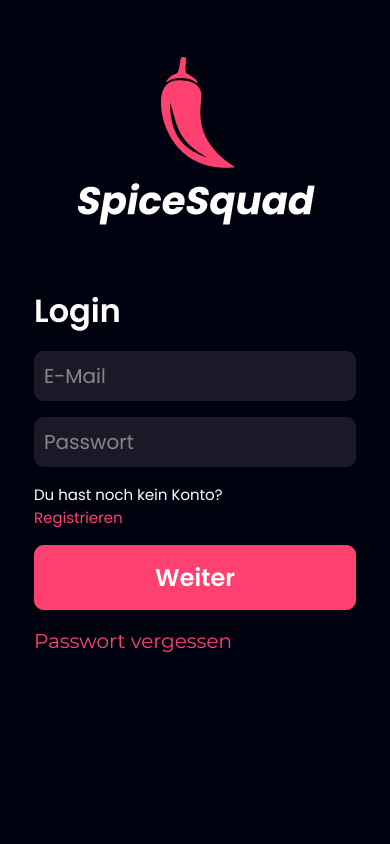
\includegraphics[height=80mm]{images/benutzeroberfläche/LoginView.jpg}
        \caption{Anmelde-Ansicht \ref{ui:LoginView}}
        \label{fig:LoginView}
    \end{minipage}
\end{figure}
\begin{figure}[htp]
    \begin{minipage}
        [t]{0.49\textwidth}
        \centering
        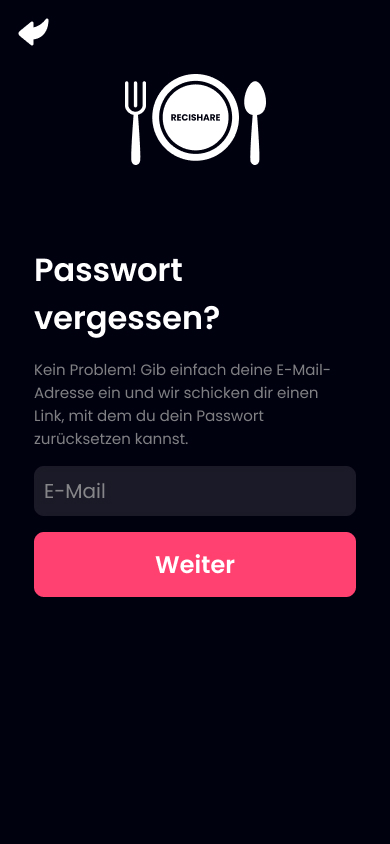
\includegraphics[height=80mm]{images/benutzeroberfläche/PasswordResetView.jpg}
        \caption{Passwort-Zurücksetzen-Ansicht \ref{ui:PasswordResetView}}
        \label{fig:PasswordResetView}
    \end{minipage}
    \begin{minipage}
        [t]{0.49\textwidth}
        \centering
        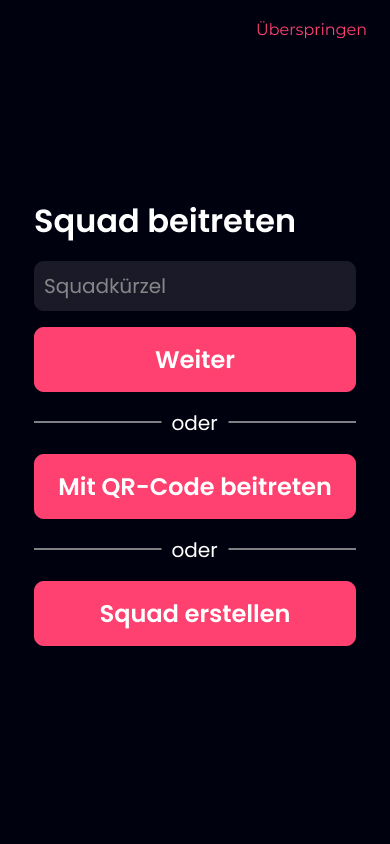
\includegraphics[height=80mm]{images/benutzeroberfläche/GroupJoiningView.jpg}
        \caption{Gruppen-Beitritts-Ansicht \ref{ui:GroupJoiningView}}
        \label{fig:GroupJoiningView}
    \end{minipage}
\end{figure}
\begin{figure}[htp]
    \begin{minipage}
        [t]{0.49\textwidth}
        \centering
        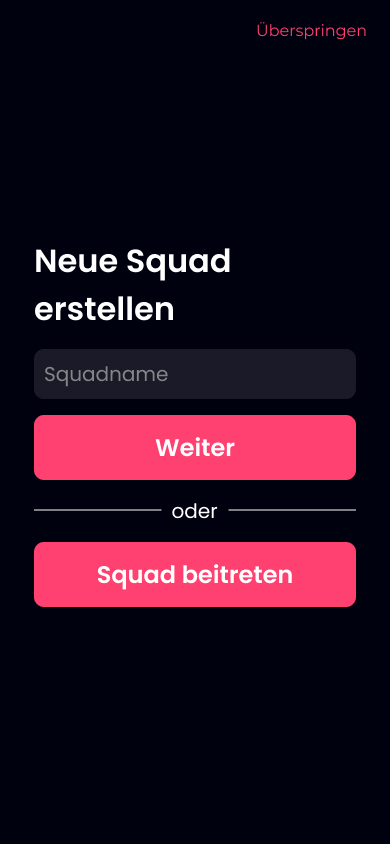
\includegraphics[height=80mm]{images/benutzeroberfläche/GroupCreationView.jpg}
        \caption{Gruppen-Erstellungs-Ansicht \ref{ui:GroupCreationView}}
        \label{fig:GroupCreationView}
    \end{minipage}
    \begin{minipage}
        [t]{0.49\textwidth}
        \centering
        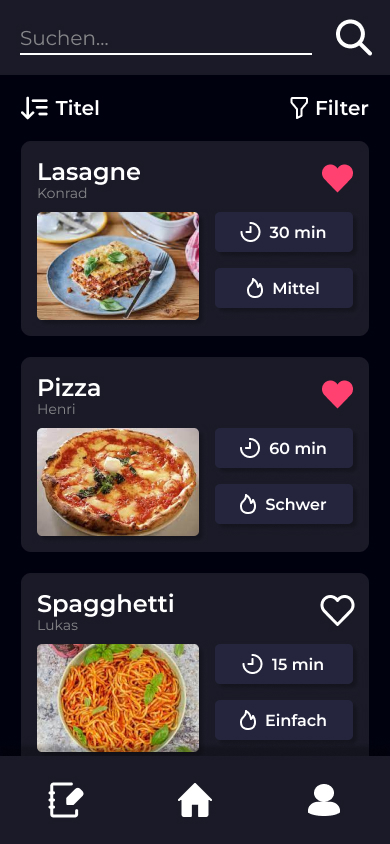
\includegraphics[height=80mm]{images/benutzeroberfläche/MainView.jpg}
        \caption{Haupt-Ansicht \ref{ui:MainView}}
        \label{fig:MainView}
    \end{minipage}
\end{figure}
\begin{figure}[htp]
    \begin{minipage}
        [t]{0.49\textwidth}
        \centering
        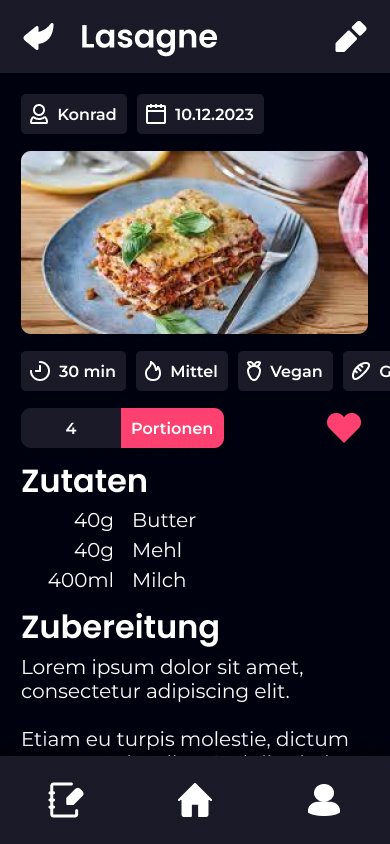
\includegraphics[height=80mm]{images/benutzeroberfläche/RecipeView.jpg}
        \caption{Rezept-Ansicht \ref{ui:RecipeView}}
        \label{fig:RecipeView}
    \end{minipage}
    \begin{minipage}
        [t]{0.49\textwidth}
        \centering
        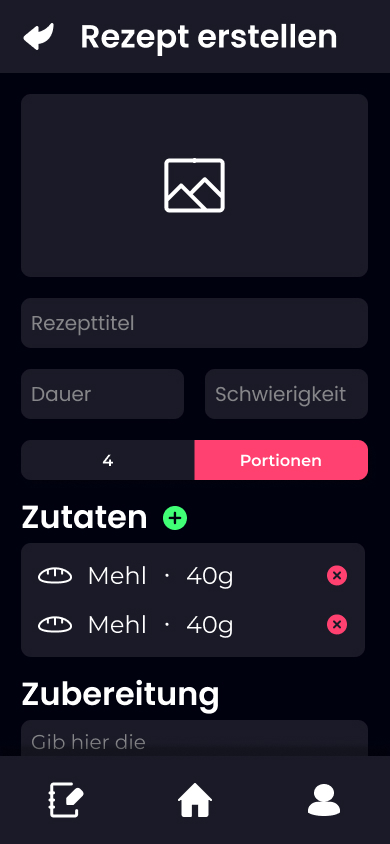
\includegraphics[height=80mm]{images/benutzeroberfläche/RecipeCreationView.jpg}
        \caption{Rezept-Erstellungs-Ansicht \ref{ui:RecipeCreationView}}
        \label{fig:RecipeCreationView}
    \end{minipage}
\end{figure}
\begin{figure}[htp]
    \begin{minipage}
        [t]{0.49\textwidth}
        \centering
        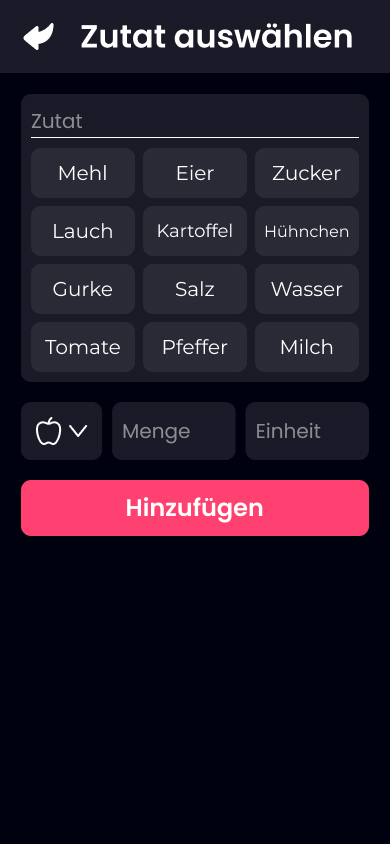
\includegraphics[height=80mm]{images/benutzeroberfläche/IngredientPickerView.jpg}
        \caption{Zutaten-Auswahl-Ansicht \ref{ui:IngredientPickerView}}
        \label{fig:IngredientPickerView}
    \end{minipage}
    \begin{minipage}
        [t]{0.49\textwidth}
        \centering
        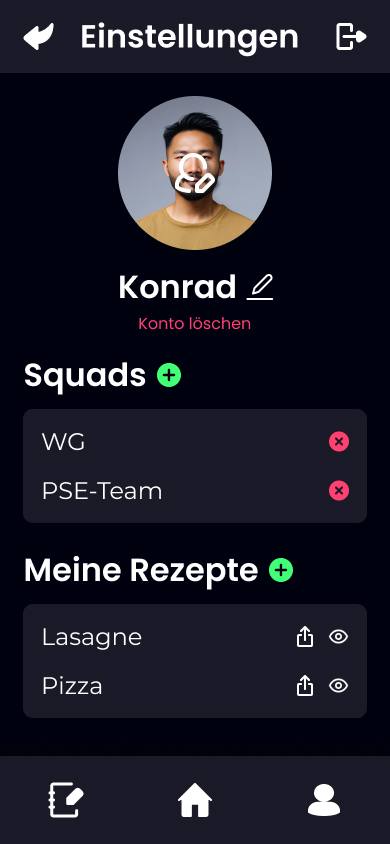
\includegraphics[height=80mm]{images/ui/SettingsView.jpg}
        \caption{Verwaltungs-Ansicht \ref{ui:SettingsView}}
        \label{fig:SettingsView}
    \end{minipage}
\end{figure}
\begin{figure}[htp]
    \begin{minipage}
        [t]{0.49\textwidth}
        \centering
        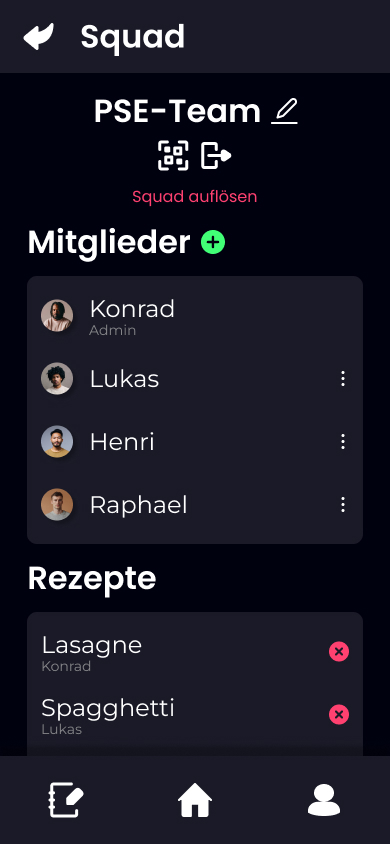
\includegraphics[height=80mm]{images/benutzeroberfläche/GroupDetailView.jpg}
        \caption{Gruppen-Detail-Ansicht \ref{ui:GroupDetailView}}
        \label{fig:GroupDetailView}
    \end{minipage}
    \begin{minipage}
        [t]{0.49\textwidth}
        \centering
        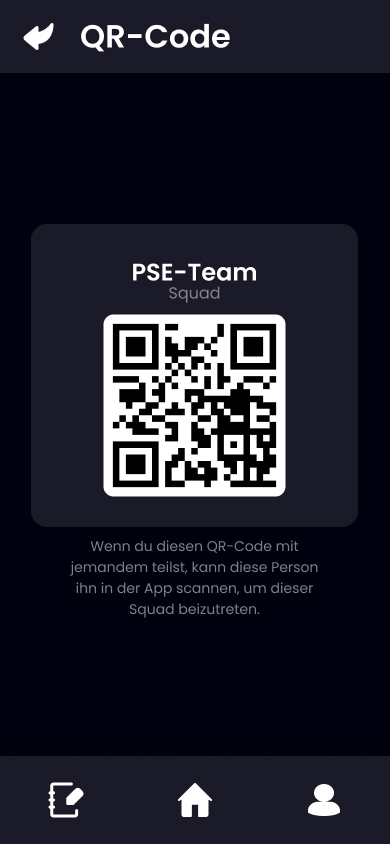
\includegraphics[height=80mm]{images/benutzeroberfläche/QRCodeView.jpg}
        \caption{QR-Code-Ansicht \ref{ui:QRCodeView}}
        \label{fig:QRCodeView}
    \end{minipage}
\end{figure}
\newpage
\renewcommand{\theparagraph}{\arabic{section}.\arabic{subsection}.\arabic{subsubsection}.\arabic{paragraph}}
\setcounter{secnumdepth}{3}

\section{Produktfunktionen}

\changelocaltocdepth{1}
\renewcommand{\thesubsection}{$\langle$F\arabic{subsection}0$\rangle$}

\subsection{Einloggen und Ausloggen}
\textbf{Anwendungsfall:} Der Nutzer möchte sich in der App anmelden und sich danach wieder abmelden.\\
\textbf{Anforderungen:} \ref{rm:Login}, \ref{rm:Logout}\\
\textbf{Ziel:} Der Nutzer erhält Zugang zu seinem Profil in der App, indem eine Verbindung zum Server hergestellt wird. Danach wird diese Verbindung wieder getrennt.\\
\textbf{Vorbedingung:} Der Nutzer hat bereits ein Konto erstellt.\\
\textbf{Nachbedingung Erfolg:} Der Nutzer ist erfolgreich ausgeloggt und wird zur Login-Ansicht der App weitergeleitet.\\
\textbf{Nachbedingung Fehlschlag:} Das Passwort oder der Nutzername ist falsch, sodass eine Fehlermeldung erscheint bei dem fehlerhaften Eingabefeld.\\
\textbf{Akteure:} Nutzer\\
\textbf{Auslösendes Ereignis:} -\\
\textbf{Beschreibung:}
\begin{enumerate}
    \item Der Nutzer startet die App.
    \item Die Login-Ansicht erscheint
    \item Der Nutzer gibt seinen Nutzernamen ein.
    \item Der Nutzer gibt sein Passwort ein.
    \item Der Nutzer klickt auf den Weiter-Button, um die Anmeldung abzuschließen.
    \item Der Nutzer klickt auf den Verwaltungsansichts-Button.
    \item Der Nutzer Klick auf den ausloggen-Button.
    \item Der Nutzer wird zur Login-Ansicht weitergeleitet
\end{enumerate}
\textbf{Alternativen:} Mit einem Klick auf den Registrieren-Button kann ein Nutzer Konto angelegt werden. Mit einem Klick auf den Passwort-vergessen-Button Knopf kann das Passwort eines bestehenden Kontos geändert werden.
\newpage

\subsection{Registrierung und Konto löschen}
\textbf{Anwendungsfall:} Der Nutzer möchte ein Nutzerkonto anlegen und danach sein Konto löschen.\\
\textbf{Anforderungen:} \ref{rm:Registering}, \ref{rs:AccountDeletion} \\
\textbf{Ziel:} Der Nutzer legt ein Nutzerkonto an, um alle Features der App nutzen zu können und löscht das Nutzerkonto danach.\\
\textbf{Vorbedingung:} -\\
\textbf{Nachbedingung Erfolg:} Der Nutzer wird zum Gruppen-Ansicht weitergeleitet und mit einem Pop-up-Fenster erfolgt die Bestätigung zur erfolgreichen Registrierung.\\
\textbf{Nachbedingung Fehlschlag:} Eine Fehlermeldung erscheint beim fehlerhaften Eingabefenster.\\
\textbf{Akteure:} Nutzer\\
\textbf{Auslösendes Ereignis:} Der Nutzer muss auf den Registrieren-Button in der Login-Ansicht klicken.\\
\textbf{Beschreibung:}
\begin{enumerate}
    \item Der Nutzer klickt auf den Registrieren-Button.
    \item Der Nutzer gibt einen Nutzernamen ein.
    \item Der Nutzer gibt seine E-Mail-Adresse ein.
    \item Der Nutzer gibt ein Passwort ein.
    \item Der Nutzer gibt das Passwort nochmals ein.
    \item Der Nutzer klickt auf den Weiter-Button.
    \item Der Nutzer wird in die Gruppen-Beitritts-Ansicht weitergeleitet.
    \item Der Nutzer klickt auf den Überspringen-Button.
    \item Der Nutzer wird zur Hauptansicht weitergeleitet.
    \item Der Nutzer klickt auf den Verwaltungsansichts-Button.
    \item Der Nutzer klickt auf den Konto-Löschen-Button.
    \item Ein Pop-up-Fenster erscheint zur Bestätigung zum Löschen des Benutzerkonto löschen.
    \item Der Nutzer klickt auf den Bestätigen-Button.
    \item Das Benutzerkonto wird gelöscht.
    \item Der Nutzer wird zur Login-Ansicht weitergeleitet.
\end{enumerate}
\textbf{Alternativen:} -
\newpage

\subsection{Passwort zurücksetzen}
\textbf{Anwendungsfall:} Der Nutzer möchte das Passwort für seinen Benutzerkonto zurücksetzen.\\
\textbf{Anforderungen:} \ref{rs:ResetPassword}\\
\textbf{Ziel:} Der Nutzer kann ein neues Passwort setzen.\\
\textbf{Vorbedingung:} Die App muss bereits gestartet worden sein.\\
\textbf{Nachbedingung Erfolg:} Der Nutzer wird zum Login-Ansicht weitergeleitet und mit einem Pop-up-Fenster erfolgt die Bestätigung der Versendung einer E-Mail an die angegeben E-Mail-Adresse.\\
\textbf{Nachbedingung Fehlschlag:} Ein Pop-up-Fenster erscheint mit einer Fehlermeldung.\\
\textbf{Akteure:} Nutzer\\
\textbf{Auslösendes Ereignis:} Der Nutzer muss auf den Passwort-vergessen-Button in der Login-Ansicht klicken.\\
\textbf{Beschreibung:}
\begin{enumerate}
    \item Klick auf den Passwort-vergessen-Button.
    \item Eingabe der E-Mail-Adresse.
    \item Klick auf den Weiter-Button.
\end{enumerate}
\textbf{Alternativen:} Durch das Klicken auf den Verlassen-Button wird der Nutzer zurück zur Login-Ansicht geleitet.
\newpage


\subsection{Benutzernamen und Profilbild ändern}
\textbf{Anwendungsfall:} Der Nutzer möchte seinen Nutzernamen und sein Profilbild ändern.\\
\textbf{Anforderungen:} \ref{rs:ChangeUsername}, \ref{rc:ProfileImage}\\
\textbf{Ziel:} Der Nutzer kann seinen Benutzernamen und sein Profilbild an seine Wünsche anpassen.\\
\textbf{Vorbedingung:} -\\
\textbf{Nachbedingung Erfolg:} Der aktualisierte Nutzername und das aktualisierte Profilbild wird anderen Nutzern angezeigt.\\
\textbf{Nachbedingung Fehlschlag:} Ein Pop-up-Fenster erscheint mit einer Fehlermeldung.\\
\textbf{Akteure:} Nutzer\\

\textbf{Auslösendes Ereignis:} Der Nutzer klickt auf den Button für die Verwaltungs-Ansicht.\\
\textbf{Beschreibung:}
\begin{enumerate}
    \item Der Nutzer klickt auf den Button für die Verwaltungs-Ansicht.
    \item Der Nutzer klickt auf den Nutzernamen-bearbeiten-Button.
    \item Der neue Nutzername wird eingegeben.
    \item Der Nutzer klickt auf den Speichern-Button.
    \item Der Nutzer klickt auf sein Profilbild.
    \item Der Nutzer kann mit Hilfe des betriebssystemeigenen Dateimanagers ein neues Profilbild aussehen.
\end{enumerate}
\textbf{Alternativen:} Der Nutzer kann auch sein Profilbild komplett entfernen. Auch kann der Nutzer auf den Exit-Button klicken und der Prozess wird abgebrochen und der Nutzer gelangt zurück zur Verwaltungs-Ansicht.\\
\newpage


\subsection{Rezept erstellen, ändern und löschen}
\textbf{Anwendungsfall:} Der Nutzer möchte ein neues Rezept erstellen, es danach ändern und es schließlich löschen.\\
\textbf{Anforderungen:} \ref{rm:RecipeCreation}, \ref{rm:RecipeContents}, \ref{rm:RecipeManagement}, \ref{rc:Images}, \ref{rc:IngredientList}\\
\textbf{Ziel:} Der Nutzer erstellt ein Rezept, welches er mit seinen Gruppen teilen möchte, oder auch nur für sich sichtbar macht. Nimmt dann Änderungen vor, um es dann wieder zu löschen.\\
\textbf{Vorbedingung:} -\\
\textbf{Nachbedingung Erfolg:} Das erstellte und geänderte Rezept wird in der Verwaltungsansicht nicht mehr angezeigt.  \\
\textbf{Nachbedingung Fehlschlag:} Ein Pop-up-Fenster erscheint mit einer Fehlermeldung.\\
\textbf{Akteure:} Nutzer\\
\textbf{Auslösendes Ereignis:} In der Haupt-Ansicht klickt der Nutzer auf den neues-Rezept -anlegen-Button.\\

\textbf{Beschreibung:}
\begin{enumerate}
    \item Der Nutzer klickt auf den Button für ein neues Rezept.
    \item Der Nutzer gib den Rezepttitel, die Zubereitungsdauer, die Zutaten mit Mengenangaben, den Schwierigkeitsgrad, die Portionsanzahl und eine Zubereitungsanweisungen an.
    \item Der Nutzer klickt auf den Speichern-Button.
    \item Der Nutzer wird zur Haupt-Ansicht weitergeleitet.
    \item Der Nutzer klickt auf den Verwaltungs-Ansicht-Button.
    \item Der Nutzer klickt auf das gerade erstellte Rezept.
    \item Der Nutzer wird zur Rezept-Erstellungs-Ansicht weitegeleitet.
    \item Der Nutzer ändert den Rezepttitel.
    \item Der Nutzer klickt auf den Speichern-Button.
    \item Der Nutzer wird zur Haupt-Ansicht weitergeleitet.
    \item Der Nutzer klickt auf den Verwaltungs-Ansicht-Button.
    \item Der Nutzer klickt auf den Löschen-Button des gerade geänderten Rezepts.
    \item Ein Pop-up-Fenster erscheint mit der Frage zur Bestätigung, dass das Rezept gelöscht werden soll.
    \item Der Nutzer klickt auf den bestätigen Button.
    \item Dem Nutzer wird das Rezept nicht mehr angezeigt.
\end{enumerate}
\textbf{Alternativen:} Der Nutzer kann ein Bild vom fertigen Gericht können.
\newpage


\subsection{Rezept suchen, sortieren, filtern, anschauen und favorisieren}
\textbf{Anwendungsfall:} Der Nutzer möchte nach einem Rezept Suchen, dann die Rezepte nach dem Schwierigkeitsgrad filtern, ein Rezept sich genauer anschauen und dies dann favorisieren.\\
\textbf{Anforderungen:} \ref{rm:RecipeViewing}, \ref{rs:RecipeFavourites}, \ref{rs:PortionScaling}, \ref{rs:Searching}, \ref{rc:Filtering}, \ref{rc:Sorting}, \ref{rc:PDFExport}\\
\textbf{Ziel:} Der Nutzer kann mit dem Suchen, dem Filtern und dem Favorisieren sein gewünschtes Rezept schnell finden und es mithilfe der Zubereitungsanweisungen nachvollziehen.\\
\textbf{Vorbedingung:} Dem Nutzer wird mindestens ein Rezept in der Haupts-Ansicht oder in der Gruppen-Detail-Ansicht angezeigt.\\
\textbf{Nachbedingung Erfolg:} Das Rezept favorisierte Rezept ist mit den anderen favorisierten Rezepten beim Filter favorisierte Rezepte auffindbar.\\
\textbf{Nachbedingung Fehlschlag:} Ein Pop-up-Fenster erscheint mit einer Fehlermeldung.\\
\textbf{Akteure:} Nutzer\\
\textbf{Auslösendes Ereignis:} Klick auf die Suchzeile in der Haupt-Ansicht.\\
\textbf{Auslösendes Ereignis:} Klick auf die Suchzeile in der Hauptansicht.\\
\textbf{Beschreibung:}
\begin{enumerate}
    \item Der Nutzer klickt auf die Suchzeile.
    \item Der Nutzer klickt auf den Sortierungs-methode-Button und wählt Hinzufügedatum aus.
    \item Der Nutzer klickt auf den Filtern-nach-Button und wählt Schwierigkeitsgrad Mittel.
    \item Der Nutzer gibt einen Suchbegriff ein.
    \item Der Nutzer klickt auf das erste Rezept.
    \item Der Nutzer wird zur Rezeptansicht weitergeleitet.
    \item Der Nutzer skaliert das Rezept auf eine Person.
    \item Der Nutzer klickt auf den Favoriten-Button.
\end{enumerate}

\textbf{Erweiterung:} Der Nutzer kann die voreingestellte Portionsgröße auf die gewünschte Anzahl ändern. Des Weiteren kann ein Rezept auch in der Form eines PDFs exportiert werden.\\
\textbf{Alternativen:} -
\newpage

\subsection{Gruppe erstellen und Gruppe auflösen}
\textbf{Anwendungsfall:} Der Nutzer möchte eine neue Gruppe erstellen, mit der die Rezepte geteilt werden können und diese danach wieder auflösen.\\
\textbf{Anforderungen:} \ref{rm:GroupCreation}, \ref{rm:GroupAdmin}, \ref{rm:GroupDeletion} \\
\textbf{Ziel:} Der Nutzer kann mit der neuen Gruppe seine Rezepte teilen und danach die Gruppe auch wieder auflösen.\\
\textbf{Vorbedingung:} -\\
\textbf{Nachbedingung Erfolg:} Die erstellte Gruppe wird in der Verwaltung-Ansicht nicht mehr angezeigt und der Administrator Status des Nutzers wird wieder entfernt.\\
\textbf{Nachbedingung Fehlschlag:} Ein Pop-up-Fenster erscheint mit einer Fehlermeldung.\\
\textbf{Akteure:} Nutzer\\

\textbf{Auslösendes Ereignis:} Der Nutzer klickt auf den Gruppe-erstellen-Button.\\
\textbf{Beschreibung:}
\begin{enumerate}
    \item Der Nutzer klickt auf den Gruppe-erstellen-Button.
    \item Der Nutzer wird zur Gruppen-Erstellungs-Ansicht weitergeleitet.
    \item Der Nutzer gibt den Gruppennamen ein.
    \item Der Nutzer klickt auf den Speichern-Button.
    \item Der Nutzer wird zur Verwaltungs-Ansicht zurückgeleitet.
    \item Der Nutzer klickt auf die Gruppe und wird zur Gruppen-Detail-Ansicht weitergeleitet.
    \item Der Nutzer klickt auf den Gruppen-auflösen-Button.
    \item Ein Pop-up-Fenster erscheint, welches um Bestätigung bitten.
    \item Der Nutzer klickt auf den Button zum Bestätigen.
    \item Der Nutzer wird zur Verwaltungsansicht weitergeleitet.
\end{enumerate}
\textbf{Alternativen:} Mit dem Gruppe-beitreten-Button kann auch zur Gruppen-Erstellungs-Ansicht gelangt werden.
\newpage


\subsection{Gruppe beitreten und verlassen}
\textbf{Anwendungsfall:} Der Nutzer möchte einer neuen Gruppe beitreten und diese danach verlassen.\\
\textbf{Anforderungen:} \ref{rm:GroupJoining} \\
\textbf{Ziel:} Der Nutzer ist der Gruppe beigetreten und kann alle in der Gruppe geteilten Rezepte ansehen und diese auch wieder verlassen, sodass in der Hauptansicht die Rezepte nicht mehr angezeigt werden.\\
\textbf{Vorbedingung:} -\\
\textbf{Nachbedingung Erfolg:} Die beigetretene Gruppe wird nicht mehr in der Verwaltung-Ansicht angezeigt und die Rezepte der Gruppe werden nicht mehr in der Hauptansicht angezeigt.\\
\textbf{Nachbedingung Fehlschlag:} Ein Pop-up-Fenster erscheint mit einer Fehlermeldung.\\
\textbf{Akteure:} Nutzer\\
\textbf{Auslösendes Ereignis:} Klick auf den Gruppe-beitreten-Button.\\

\textbf{Beschreibung:}\\
\begin{enumerate}
    \item Der Nutzer klickt auf den Gruppe-beitreten-Button in der Verwaltung-Ansicht.
    \item Der Nutzer gibt das Gruppenkürzels ein.
    \item Der Nutzer klickt auf den Gruppe-beitreten-Button.
    \item Der Nutzer wird zur Gruppen-Detail-Ansicht weitergeleitet.
    \item Der Nutzer klickt auf den Gruppe-verlassen-Button.
    \item Ein Pop-up-Fenster erscheint, welches um Bestätigung bitten.
    \item Der Nutzer klickt auf den Button zum Bestätigen.
    \item der Nutzer wird zur Verwaltungsansicht weitergeleitet.
\end{enumerate}
\textbf{Erweiterung:}\\
\textbf{Alternativen:} Nach dem Login-Ansicht wird man zur Gruppe-beitreten-Ansicht weitergeleitet, wodurch auch einer Gruppe beigetreten werden kann. Einer Gruppe kann auch mit dem Scannen eines QR-Codes beigetreten werden ohne die Eingabe eines Gruppennamens.
\newpage


\subsection{Gruppenkürzel ausgeben}
\textbf{Anwendungsfall:} Der Nutzer möchte den Gruppenkürzel erhalten.\\
\textbf{Anforderungen:} \ref{rm:GroupId}\\
\textbf{Ziel:} Der Nutzer kann die Daten der Gruppe mit anderen Nutzern teilen, um diese die Möglichkeit zu geben der Gruppe beizutreten.\\
\textbf{Vorbedingung:} Der Nutzer ist in einer Gruppe Mitglied.\\
\textbf{Nachbedingung Erfolg:} Ein Pop-up-Fenster erscheint mit den Daten der Gruppe.\\
\textbf{Nachbedingung Fehlschlag:} Ein Pop-up-Fenster erscheint mit einer Fehlermeldung.\\
\textbf{Akteure:} Nutzer \\
\textbf{Auslösendes Ereignis:} Der Nutzer klickt in der Verwaltungs-Ansicht auf die Gruppe und wird zur Gruppen-Detail-Ansicht weitergeleitet.\\
\textbf{Beschreibung:}
\begin{enumerate}
    \item Der Nutzer klickt auf die Gruppen-Detail-Ansicht-Button.
    \item Der Nutzer klickt auf den Gruppen-Informations-Button.
    \item Der Nutzer wird zur QR-Code-Ansicht weitergeleitet.
    \item Der Nutzer sieht den QR-Code, der alle Informationen enthält.
\end{enumerate}
\textbf{Alternativen:} -
\newpage


\subsection{Administrator ernennen und Administratorenstatus entfernen}
\textbf{Anwendungsfall:} Der Nutzer möchte ein weiteres Mitglied der Gruppe zu einem Administrator der Gruppe ernennen und dem Nutzer den Administrator Status dann wieder aberkennen.\\
\textbf{Anforderungen:} \ref{RS3}\\
\textbf{Ziel:} Der Nutzer kann seine Rechte für die Gruppe mit anderen Mitgliedern teilen und auch anderen Mitglieder die Rechte entziehen.\\
\textbf{Vorbedingung:} Der Nutzer ist Administrator der Gruppe.\\
\textbf{Nachbedingung Erfolg:} Ein weiteres Mitglied besitze die gegebenen Rechte nicht mehr.\\
\textbf{Nachbedingung Fehlschlag:} Ein Pop-up-Fenster erscheint mit einer Fehlermeldung.\\
\textbf{Akteure:} Nutzer \\

\textbf{Auslösendes Ereignis:} Klick auf die Detail-Ansicht eines Mitglieds der Gruppe.\\
\textbf{Beschreibung:}
\begin{enumerate}
    \item Der Nutzer klickt auf die Detail-Ansicht eines Mitglieds der Gruppe.
    \item Der Nutzer klickt auf die Option den Nutzer zum Administrator der Gruppe zu ernennen.
    \item Ein Pop-up-Fenster erscheint mit einer Bestätigung, dass der Nutzer zum Administrator der Gruppe ernannt wurde.
    \item Der Nutzer klickt auf die Detail-Ansicht eines Mitglieds der Gruppe.
    \item Der Nutzer klickt auf die Option den Nutzer die Administrator Rechte der Gruppe zu entziehen.
    \item Ein Pop-up-Fenster erscheint mit einer Bestätigung, dass dem Nutzer die Administrator Rechte entzogen worden.
\end{enumerate}
\textbf{Alternativen:} -
\newpage

\subsection{Nutzer kicken und Nutzer bannen}
\textbf{Anwendungsfall:} Ein Administrator möchte ein Mitglied der Gruppe aus der Gruppe kicken und ein anderes Mitglied aus der Gruppe bannen und danach wieder entbannen.\\
\textbf{Anforderungen:} \ref{RS4}\\
\textbf{Ziel:} Ein Administrator möchte das erste Mitglied nur aus der Gruppe kicken und dem zweiten Mitglied nicht mehr die Möglichkeit bieten der Gruppe beizutreten.\\
\textbf{Vorbedingung:} Der Nutzer ist Administrator der Gruppe und die Gruppe hat insgesamt mindestens drei Mitglieder.\\
\textbf{Nachbedingung Erfolg:} Die beiden Nutzer sind nicht mehr in der Gruppe.\\
\textbf{Nachbedingung Fehlschlag:} Ein Pop-up-Fenster erscheint mit einer Fehlermeldung.\\
\textbf{Akteure:} Nutzer\\
\textbf{Auslösendes Ereignis:} Der Nutzer klickt auf die Detail-Ansicht des Mitglieds der Gruppe.\\
\textbf{Beschreibung:}
\begin{enumerate}
    \item Der Nutzer klickt auf die Detail-Ansicht des ersten Mitglieds der Gruppe.
    \item Der Nutzer klickt auf die Option den Nutzer zu kicken.
    \item Ein Pop-up-Fenster erscheint mit einer Bitte um Bestätigung, dass der Nutzer gekickt werden soll.
    \item Der Nutzer klickt auf den Bestätigen-Button.
    \item Der Nutzer klickt auf die Detail-Ansicht des zweiten Mitglieds der Gruppe.
    \item Der Nutzer klickt auf die Option den Nutzer zu bannen.
\end{enumerate}
\textbf{Alternativen:} -
\newpage


\subsection{Rezepte verwalten für die Gruppen}
\textbf{Anwendungsfall:} Der Nutzer meldet ein Rezept, welches mit der Gruppe von einem Nutzer geteilt wird, und der Administrator der Gruppe will dieses Rezept, ausblenden und danach die Ausblendung wieder rückgängig machen.\\
\textbf{Anforderungen:} \ref{RS5}, \ref{RC9}\\
\textbf{Ziel:} Der Administrator kann bestimmen welche Rezepte den Mitgliedern und ihm selbst angezeigt werden.\\
\textbf{Vorbedingung:} Der Nutzer und der Administrator sind in einer Gruppe und in der Gruppe bestehen Rezepte.\\
\textbf{Nachbedingung Erfolg:} Das Rezept wird wieder Haupt-Ansicht oder in der Gruppen-Detail-Ansicht angezeigt, nach dem es für die Mitglieder ausgeblendet war.\\
\textbf{Nachbedingung Fehlschlag:} Ein Pop-up-Fenster erscheint mit einer Fehlermeldung.\\
\textbf{Akteure:} Nutzer, Administrator  \\

\textbf{Auslösendes Ereignis:} Der Nutzer klickt in der Gruppen-Detail-Ansicht auf den ausblenden-Button von einem Rezept.\\
\textbf{Beschreibung:}
\begin{enumerate}
    \item Der Nutzer klickt in der Gruppen-Detail-Ansicht auf den Melden-Button von einem Rezept.
    \item Ein Pop-up-Fenster erscheint, welches um Bestätigung bittet, dass das Rezept wirklich gemeldet werden soll.
    \item Der Nutzer klickt auf den Bestätigen-Button.
    \item Der Administrator erhält eine E-Mail mit der Benachrichtigung über die Meldung des Rezepts.
    \item Der Administrator öffnet die App und manövriert zur Gruppen-Detail-Ansicht.
    \item Der Administrator klickt in der Gruppen-Detail-Ansicht auf den Ausblenden-Button von einem Rezept.
    \item Ein Pop-up-Fenster erscheint, welches um Bestätigung bittet, dass das Rezept wirklich ausgeblendet werden soll.
    \item Der Administrator klickt auf den Bestätigen-Button.
    \item Der Administrator wird zum Gruppen-Detail-Ansicht weitergeleitet.
    \item Der Administrator klickt in der Gruppen-Detail-Ansicht auf den einblenden-Button von dem ausgeblendeten Rezept.
    \item Ein Pop-up-Fenster erscheint, welches um Bestätigung bittet, dass das Rezept wirklich gemeldet werden soll.
    \item Der Administrator klickt auf den Bestätigen-Button.
    \item Der Administrator wird zum Gruppen-Detail-Ansicht weitergeleitet.
\end{enumerate}
\textbf{Alternativen:} -
\newpage


\subsection{Gruppennamen ändern}
\textbf{Anwendungsfall:} Ein Administrator möchte den Gruppennamen ändern.\\
\textbf{Anforderungen:} \ref{rc:GroupRenaming}\\

\textbf{Ziel:} Ein Administrator kann den Gruppennamen nach seinen Vorstellungen anpassen.\\
\textbf{Vorbedingung:} Der Nutzer ist Administrator der Gruppe.\\
\textbf{Nachbedingung Erfolg:} Der angepasste Gruppenname wird den Mitgliedern angezeigt.\\
\textbf{Nachbedingung Fehlschlag:} Ein Pop-up-Fenster erscheint mit einer Fehlermeldung.\\
\textbf{Akteure:} Nutzer\\
\textbf{Auslösendes Ereignis:} In der Gruppen-Detail-Ansicht wird auf den Bearbeiten-Button geklickt.\\

\textbf{Beschreibung:}
\begin{enumerate}
    \item Der Nutzer klickt auf den Bearbeiten-Button.
    \item Der Nutzer gibt den neuen Gruppennamen ein.
    \item Der Nutzer klickt auf den Bestätigen-Button.
    \item Der Nutzer wird zur Gruppen-Detail-Ansicht
\end{enumerate}
\textbf{Alternativen:} -
\newpage


\resetSubSectionNumbering


\section{Produktdaten}
\changelocaltocdepth{1}
\renewcommand{\thesubsection}{$\langle$D\arabic{subsection}0$\rangle$}

Um die App nutzen zu können, ist es erforderlich einige Daten zu speichern. Diese werden auf unterschiedlichen Geräten gespeichert:

\subsection{Smartphone-Daten}
\begin{itemize}
    \item Anwendung
    \item Konfigurationsdatei
\end{itemize}

\subsection{Server-Daten}
\begin{itemize}
    \item Rezepte
    \item Nutzerdaten
    \item Gruppen
\end{itemize}

\resetSubSectionNumbering
\section{Nichtfunktionale Anforderungen}
Im folgenden Kapitel werden die nichtfunktionalen Anforderungen und Qualitätsmerkmale der App definiert.
Anschließend werden die wichtigsten Qualitätsmerkmale operationalisiert und, falls diese nicht als allgemeine Richtlinie (z.B. Standard, Norm usw.) zu Verfügung gestellt werden,
als konkrete Produktanforderungen konkretisiert.

\subsection{Funktionalität}
\begin{tabular}{| c | c | c | c | c |}
    \hline
    \textbf{ Produktqualität } & \textbf{sehr gut} & \textbf{gut} & \textbf{normal} & \textbf{nicht relevant} \\ \hline
    Angemessenheit           & X                 &              &                 &                         \\ \hline
    Richtigkeit              &                   & X            &                 &                         \\ \hline
    Interoperabilität        & X                 &              &                 &                         \\ \hline
    Ordnungsmäßigkeit        &                   & X            &                 &                         \\ \hline
\end{tabular}

\textbf{Angemessenheit}\\
Da jede Komponente der App dem Nutzer entweder beim Teilen, Finden oder Speichern von Rezepten unterstützt, ist die Angemessenheit der App insgesamt als sehr hoch einzustufen

\textbf{Richtigkeit und Ordnungsmäßigkeit}\\
Die App bietet nur an wenigen Schnittstellen wie z.B. dem Erstellen bzw. Verändern von Rezepten Anfälligkeit für Verlust oder Verfälschung von Daten. Dennoch ist ein hohes Maß an Richtigkeit insbesondere im Bereich der Nutzer- und Rezeptverwaltung erwünscht.

\textbf{Interoperabilität}\\
Da die App mit Schnittstellen wie bspw. dem Server oder Android-Betriebssystem fehlerfrei kommunizieren muss, um korrekt zu arbeiten, ist eine sehr gute Interoperabilität wichtig.

\subsection{Sicherheit}
\begin{tabular}{| c | c | c | c | c |}
    \hline
    \textbf{Produktqualität} & \textbf{sehr gut} & \textbf{gut} & \textbf{normal} & \textbf{nicht relevant} \\ \hline
    Zuverlässigkeit         & X                 &              &                 &                         \\ \hline
    Reife                    & X                 &              &                 &                         \\ \hline
    Fehlertoleranz           &                   &              & X               &                         \\ \hline
    Wiederherstellbarkeit    &                   & ?            &                 &                         \\ \hline
\end{tabular}

\textbf{Zuverlässigkeit und Reife}\\
Durch das Durchführen von Tests während der Implementierung können Fehler früh gefunden werden und der fehlerhafte Code verbessert werden.
Durch die zahlreichen Testfälle können wir eine sehr gute Zuverlässigkeit und Reife der App gewährleisten.

\textbf{Fehlertoleranz}\\
Trotz kontinuierlichen Testens während des Entwicklungsprozesses, kann es zur Laufzeit des Spiels zu Fehlern kommen.
Das Ausmaß ist dabei von Fall zu Fall unterschiedlich.
Folglich wird die Fehlertoleranz der App als normal eingestuft.

\textbf{Wiederherstellbarkeit}
?

\subsection{Benutzbarkeit}
\begin{tabular}{| c | c | c | c | c |}
    \hline
    \textbf{Produktqualität} & \textbf{sehr gut} & \textbf{gut} & \textbf{normal} & \textbf{nicht relevant} \\ \hline
    Verständlichkeit         & X                 &              &                 &                         \\ \hline
    Erlernbarkeit            & X                 &              &                 &                         \\ \hline
    Bedienbarkeit            &                   & X            &                 &                         \\ \hline
    Effizienz                &                   & X            &                 &                         \\ \hline
    Zeitverhalten            &                   & X            &                 &                         \\ \hline
    Verbrauchsverhalten      &                   & X            &                 &                         \\ \hline
\end{tabular}

\textbf{Verständlichkeit, Erlernbarkeit und Bedienbarkeit}\\
Die App soll intuitiv zugänglich sein, um ein hürdenfreie User Experience zu garantieren.

\textbf{Effizienz, Zeitverhalten und Verbraucherverhalten}\\
Die Effizienz der App muss als gut eingestuft werden, um ein möglichst langes Nutzererlebnis trotz des begrenzen Energiespeichers des Endgerätes zu realisieren.
Um dieses Ziel zu erreichen, soll die App ein relativ geringes Verbrauchs- und Zeitverhalten haben.


\subsection{Änderbarkeit}
\begin{tabular}{| c | c | c | c | c |}
    \hline
    \textbf{Produktqualität} & \textbf{sehr gut} & \textbf{gut} & \textbf{normal} & \textbf{nicht relevant} \\ \hline
    Analysierbarkeit         & X                 &              &                 &                         \\ \hline
    Modifizierbarkeit        & X                 &              &                 &                         \\ \hline
    Stabilität               &                   & X            &                 &                         \\ \hline
    Prüfbarkeit              & X                 &              &                 &                         \\ \hline
    Übertragbarkeit          &                   &              & X               &                         \\ \hline
    Anpassbarkeit            & X                 &              &                 &                         \\ \hline
    Installierbarkeit        &                   & X            &                 &                         \\ \hline
    Konformität              &                   &              & X               &                         \\ \hline
    Austauschbarkeit         & X                 &              &                 &                         \\ \hline
\end{tabular}

\textbf{Analysierbarkeit, Modifizierbarkeit, Prüfbarkeit, Anpassbarkeit und Austauschbarkeit} \newline
Analysierbarkeit, Modifizierbarkeit, Prüfbarkeit, Anpassbarkeit und Austauschbarkeit sind für späteres Erweitern und Verbessern der App unerlässlich und werden deshalb mit sehr gut eingestuft.

\textbf{Stabilität}\newline
Inhaltliche und designtechnische Änderungen der App dürfen keine Beeinträchtigung auf die Funktionalität der App haben.
Dadurch muss die Stabilität der App mit gut eingestuft werden.

\textbf{Installierbarkeit}\newline
Um die App spielen zu können, muss die App auf dem Android-Smartphone des Nutzers installiert werden.
Dadurch ist eine gute Installierbarkeit unerlässlich.

\textbf{Konformität}\newline
Die App basiert auf wenigen, klar definierten Schnittstellen. Das Verhalten und die Laufzeit auf einem Gerät beeinflusst das Verhalten nur geringfügig. Die Anforderung an die Konformität kann also als normal eingestuft werden

\subsection{Qualitätsanforderungen}
Die oben als am wichtigsten bezeichneten Qualitätsmerkmale werden im Folgenden operationalisiert, d.h. in konkreten Produktanforderungen konkretisiert oder es wird angegeben, welche Richtlinie (z. B. Standard, Norm) einzuhalten ist.

\begin{enumerate}[start=1,label={$\langle$\bfseries Q\arabic*$\rangle$}, leftmargin = 5em, itemsep=4pt, parsep=4pt]
    \item ?
    \item ?
    \item ?
\end{enumerate}

\section{Technische Produktumgebung}
In diesem Kapitel wird die technische Umgebung des Produktes beschrieben.

\subsection{Software}
\begin{itemize}
    \item Entwicklungsumgebung - Android Studio, IntelliJ
    \item UI-Entwicklungs-Kit - Flutter
    \item Implementierungssprache der App - Dart
    \item Nutzerverwaltung - Firebase
    \item Client-Betriebssystem - Android 8.0 oder eine neuere Android-Version
    \item Implementierungssprache des Servers - ?
\end{itemize}

\subsection{Hardware}
\begin{itemize}
    \item Standard-Smartphone mit Android Betriebssystem
\end{itemize}

%Todo Produktumgebung weiter ausführen
\subsection{Produktschnittstellen}
Die Benutzerschnittstelle wird über ein GUI zur Verfügung gestellt.
Das Scannen von QR-Codes ist durch die Smartphone-Kamera möglich.
\newpage

\section{Glossar}
\printglossary[type=\acronymtype]
\end{document}
